\documentclass[11pt]{exam} 
\usepackage{answers, amsthm, amsmath, amssymb, mathrsfs} \pagestyle{head} \firstpageheader{Math 228}{\bf Practice Problems 3: Graph Theory\\ Hints and Answers}{Spring 2013} \Newassociation{answer}{Ans}{Practice03-GraphTheory-solutions} 
 \def\d{\displaystyle}
\def\?{\reflectbox{?}}
\def\b#1{\mathbf{#1}}
\def\f#1{\mathfrak #1}
\def\c#1{\mathcal #1}
\def\s#1{\mathscr #1}
\def\r#1{\mathrm{#1}}
\def\N{\mathbb N}
\def\Z{\mathbb Z}
\def\Q{\mathbb Q}
\def\R{\mathbb R}
\def\C{\mathbb C}
\def\F{\mathbb F}
\def\A{\mathbb A}
\def\X{\mathbb X}
\def\E{\mathbb E}
\def\O{\mathbb O}
\def\U{\mathcal U}
\def\pow{\mathcal P}
\def\inv{^{-1}}
\def\nrml{\triangleleft}
\def\st{:}
\def\~{\widetilde}
\def\rem{\mathcal R}
\def\sigalg{$\sigma$-algebra }
\def\Gal{\mbox{Gal}}
\def\iff{\leftrightarrow}
\def\Iff{\Leftrightarrow}
\def\land{\wedge}
\def\And{\bigwedge}
\def\AAnd{\d\bigwedge\mkern-18mu\bigwedge}
\def\Vee{\bigvee}
\def\VVee{\d\Vee\mkern-18mu\Vee}
\def\imp{\rightarrow}
\def\Imp{\Rightarrow}
\def\Fi{\Leftarrow}

%\def\={\equiv}
\def\var{\mbox{var}}
\def\mod{\mbox{Mod}}
\def\Th{\mbox{Th}}
\def\sat{\mbox{Sat}}
\def\con{\mbox{Con}}
\def\bmodels{=\joinrel\mathrel|}
\def\iffmodels{\bmodels\models}
\def\dbland{\bigwedge \!\!\bigwedge}
\def\dom{\mbox{dom}}
\def\rng{\mbox{range}}
\DeclareMathOperator{\wgt}{wgt}


\def\bar{\overline}


\newcommand{\vtx}[2]{node[fill,circle,inner sep=0pt, minimum size=4pt,label=#1:#2]{}}
\newcommand{\va}[1]{\vtx{above}{#1}}
\newcommand{\vb}[1]{\vtx{below}{#1}}
\newcommand{\vr}[1]{\vtx{right}{#1}}
\newcommand{\vl}[1]{\vtx{left}{#1}}
\renewcommand{\v}{\vtx{above}{}}

\def\circleA{(-.5,0) circle (1)}
\def\circleAlabel{(-1.5,.6) node[above]{$A$}}
\def\circleB{(.5,0) circle (1)}
\def\circleBlabel{(1.5,.6) node[above]{$B$}}
\def\circleC{(0,-1) circle (1)}
\def\circleClabel{(.5,-2) node[right]{$C$}}
\def\twosetbox{(-2,-1.4) rectangle (2,1.4)}
\def\threesetbox{(-2.5,-2.4) rectangle (2.5,1.4)}
\newcommand{\twoline}[2]{\begin{pmatrix}#1 \\ #2 \end{pmatrix}}

\usepackage{tikz, multicol}
\renewenvironment{Ans}[1]{\setcounter{question}{#1}\addtocounter{question}{-1}\question }{}
\begin{document}
 \begin{questions}
\begin{Ans}{1}
		This is asking for the number of edges in $K_{10}$.  Each vertex (person) has degree (shook hands with) 9 (people).  So the sum of the degrees is $90$.  However, the degrees count each edge (handshake) twice, so there are 45 edges in the graph.  That is how many handshakes took place.%If 10 people each shake hands with each other, how many handshakes took place?  What does this question have to do with graph theory?
	
\end{Ans}
\begin{Ans}{2}
		It is possible for everyone to be friends with exactly 2 people - you could arrange the 5 people in a circle and say that everyone is friends with the two people on either side of them (so you get the graph $C_5$).  However, it is not possible for everyone to be friends with 3 people - that would lead to a graph with an odd number of odd degree vertices which is impossible - the sum of the degrees must be even.  %Among a group of 5 people, is it possible for everyone to be friends with exactly 2 of the people in the group?  What about 3 of the people in the group?
	
\end{Ans}
\begin{Ans}{3}
		This is a question about finding Euler paths.  Draw a graph with a vertex in each state, and connect vertices if their states share a border.  Exactly two vertices will have odd degree - the vertices for Nevada and Utah.  Thus you must start your road trip at in one of those states and end it in the other. %You and your friends want to tour the southwest by car.  You will visit the nine states below, with the following rather odd rule: you must cross each border between neighboring states exactly once (so, for example, you must cross the Colorado-Utah border exactly once).  Can you do it?  If so, does it matter where you start your road trip?  What fact about graph theory solves this problem?
	
\end{Ans}
\begin{Ans}{4}
		The first and the third graphs are the same, but the middle graph is different.
	
\end{Ans}
\begin{Ans}{5}
		The first (and third) graphs contain an Euler path.  All the graphs are planar.
	
\end{Ans}
\begin{Ans}{6}
		Yes.  For example, both graphs below contain 6 vertices, 7 edges, and have degrees (2,2,2,2,3,3).
		\begin{center}
		  \hfill
		  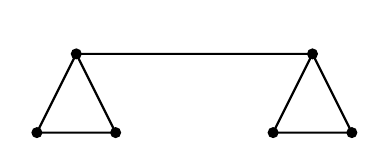
\begin{tikzpicture}
		   \draw[thick] (-2,0) \v -- (-1,0) \v -- (-1.5,1) \v -- (-2,0) (-1.5,1) -- (1.5, 1) \v -- (1,0) \v -- (2,0) \v -- (1.5,1);
		  \end{tikzpicture}
		  \hfill
		  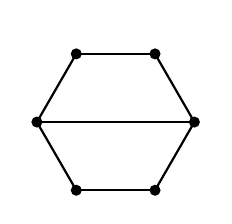
\begin{tikzpicture}
		  \foreach \x in {0,...,5}
		    \draw[thick] (\x*60:1) \v -- (\x*60 + 60:1);
		    \draw[thick] (0:1) -- (180:1);
		  \end{tikzpicture}
		  \hfill ~
		\end{center}
	
\end{Ans}
\begin{Ans}{7}
		\begin{parts}
		  \part $K_4$ does not have an Euler path or circuit.
		  \part $K_5$ has an Euler circuit (so also an Euler path).
		  \part $K_{5,7}$ does not have an Euler path or circuit.
		  \part $K_{2,7}$ has an Euler path but not an Euler circuit.
		  \part $C_7$ has an Euler circuit (it is a circuit graph!)
		  \part $P_7$ has an Euler path but no Euler circuit.
		\end{parts}
	
\end{Ans}
\begin{Ans}{8}
		When $n$ is odd, $K_n$ contains an Euler circuit.  This is because every vertex has degree $n-1$, so an odd $n$ results in all degrees being even.%For which $n$ does the graph $K_n$ contain an Euler circuit?  Explain.
	
\end{Ans}
\begin{Ans}{9}
		If both $m$ and $n$ are even, then $K_{m,n}$ has an Euler circuit.  When both are odd, there is no Euler path or circuit.  If one is 2 and the other is odd, then there is an Euler path but not an Euler circuit. %For which $m$ and $n$ does the graph $K_{m,n}$ contain an Euler path?  An Euler circuit?  Explain
	
\end{Ans}
\begin{Ans}{10}
		Three of the graphs are bipartite.  The one which is not is $C_7$ (second from the right).
	
\end{Ans}
\begin{Ans}{11}
		$C_n$ is bipartite if and only if $n = 1$ or is even.
	
\end{Ans}
\begin{Ans}{12}
		For example, $K_5$.
	
\end{Ans}
\begin{Ans}{13}
		For example, $K_{3,3}$.
	
\end{Ans}
\begin{Ans}{14}
		No.  A (connected) planar graph must satisfy Euler's formula: $V - E + F = 2$.  Here $V - E + F = 6 - 10 + 5 = 1$. %Is it possible for a planar graph to have 6 vertices, 10 edges and 5 faces?  Explain.
	
\end{Ans}
\begin{Ans}{15}
		Yes.  According to Euler's formula it would have 2 faces.  It does.  The only such graph is $C_{10}$. %If a graph has 10 vertices and 10 edges and contains an Euler circuit, must it be planar?  How many faces would it have?
	
\end{Ans}
\begin{Ans}{16}
		$G$ has 10 edges.  It could be planar, and then it would have 6 faces. %The graph $G$ has 6 vertices with degrees $2, 2, 3, 4, 4, 5$.  How many edges does $G$ have?  Could $G$ be planar?  If so, how many faces would it have.
	
\end{Ans}
\begin{Ans}{17}
		2, since the graph is bipartite.  One color for the top set of vertices, another color for the bottom set of vertices.  %What is the smallest number of colors you need to properly color the vertices of $K_{4,5}$.  That is, find the chromatic number of the graph.
	
\end{Ans}
\begin{Ans}{18}
		For example, $K_6$.  If the chromatic number is 6, then the graph is not planar - the 4-color theorem states that all planar graphs can be colored with 4 or fewer colors. %Draw a graph with chromatic number 6 (i.e., which requires 6 colors to properly color the vertices).  Could your graph be planar?  Explain.
	
\end{Ans}
\begin{Ans}{19}
		The chromatic numbers are 2, 3, 4, 5, and 3 respectively from left to right. %Find the chromatic number of each of the following graphs.
	
\end{Ans}
\begin{Ans}{20}
		\begin{parts}
		  \part Only if $n \ge 6$ and is even.%For which values of $n$ does this make sense?
		  \part None. %For which values of $n$ does the graph have an Euler path?
		  \part 12. Such a graph would have $\frac{5n}{2}$ edges.  If the graph is planar, then $n - \frac{5n}{2} + F = 2$ so there would be $\frac{4+3n}{2}$ faces.  Also, we must have $3F \le 2E$, since the graph is simple.  So we must have $3\frac{4 + 3n}{2} \le 5n$.  Solving for $n$ gives $n \ge 12$.%What is the smallest value of $n$ for which the graph might be planar? (tricky)
		\end{parts}
	
\end{Ans}
 \end{questions} \par \end{document}
